\documentclass[12pt]{article}

\usepackage[margin=1in]{geometry} % 1-inch margins
\usepackage{times}                % Times (Times New Roman–like) font
\usepackage{fancyhdr}             % For custom headers/footers
\usepackage{setspace}             % For spacing
\usepackage{titlesec}             % For section formatting
\usepackage{enumitem}             % For list alignment
\usepackage{graphicx}             % For including images
\usepackage{amsmath}              % For mathematical formatting
\usepackage{caption}              % For better figure captions
\usepackage{float}

\pagestyle{fancy}
\fancyhf{} % Clear default header and footer

% Header on the right side
\fancyhead[R]{Ultrasound Nerve Imaging And Clinical Decision Support System}

% Footer on the left side
\fancyfoot[L]{Pillai HOC College of Engineering \& Technology, Rasayani}
\fancyfoot[R]{\thepage} % Ensure page number is displayed on the right footer

% Horizontal lines in header & footer
\renewcommand{\headrulewidth}{0.4pt} 
\renewcommand{\footrulewidth}{0.4pt} 

% Set the page number to start from 18
\setcounter{page}{25}

% Number figures within subsections (e.g., Figure 5.1.1, 5.2.1)
\numberwithin{figure}{subsection}

\begin{document}

\vspace*{\fill}

\begin{center}
    {\Large \bf Chapter 5} \\[1em] % Line break with extra space (1em)
    {\Large \bf Project Analysis}
\end{center}
\vspace*{\fill}

\newpage

% Set section counter to 5 so that it starts as Chapter 5
\setcounter{section}{5}

% SUBSECTION 5.1: USE CASE DIAGRAM
\subsection{Use Case Diagram}
\vspace{50pt}

\begin{figure}[h]
\centering
    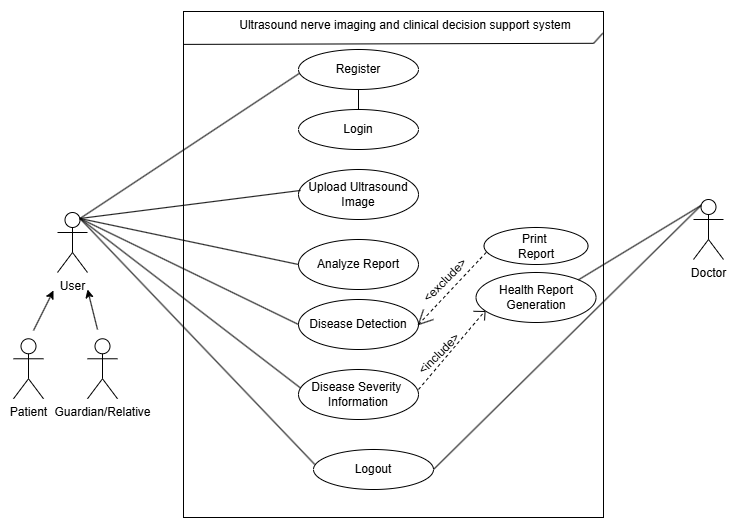
\includegraphics[width=1.0\textwidth]{usecase11.drawio.png}  % Replace with actual image filename
    \caption{Use Case Diagram}
    \label{fig:usecase}
\end{figure}

\newpage

% SUB-SUBSECTION 5.1.1: Use Case Document
\subsubsection{Use Case Document}
\vspace{10pt}

1. \textbf{Use Case: Ultrasound Nerve Imaging And Clinical Decision Support System}  \vspace{5pt}\\  
2. \textbf{Actors:} User (Patient, Doctor), System  \vspace{5pt} \\  
3. \textbf{Goal:} To analyze ultrasound images, detect diseases, generate reports, and provide clinical decision support. \vspace{5pt} \\  
4. \textbf{Main Scenario:}  
\begin{itemize}  
    \item The user registers and logs into the system.  
    \item The user uploads an ultrasound image for analysis.  
    \item The system preprocesses the image and segments it using CNN.  
    \item The system identifies nerve structures and performs disease detection using YOLOv11.  
    \item If a disease is detected, the system generates a report and provides clinical recommendations.  
    \item If no disease is found, the system updates the user with a normal health report.  
    \item The user can send the report to a hospital for further consultation.  
    \item The system offers disease condition information, doctor recommendations, and health tips.  
    \item The user can log out after viewing the report and recommendations.  
\end{itemize}  

\newpage
\subsubsection{Use Case Analysis}

\begin{enumerate}
    \item \textbf{Use Case 1: Ultrasound Image Processing and Disease Detection}  
    \begin{itemize}
        \item \textbf{Actors:} User (Patient/Doctor), System  
        \item \textbf{Goal:} To process ultrasound images and detect diseases  
        \item \textbf{Main Scenario:}
        \begin{enumerate}
            \item The user uploads an ultrasound image.  
            \item The system preprocesses the image to enhance quality.  
            \item A CNN-based model segments the image to identify key structures.  
            \item The YOLOv11 model analyzes the segmented image and detects diseases.  
            \item If a disease is detected, the system proceeds to report generation.  
            \item If no disease is found, the system updates the user accordingly.  
        \end{enumerate}
    \end{itemize}

    \item \textbf{Use Case 2: Health Report Generation and Analysis}  
    \begin{itemize}
        \item \textbf{Actors:} System  
        \item \textbf{Goal:} To generate a comprehensive health report based on the detection results  
        \item \textbf{Main Scenario:}
        \begin{enumerate}
            \item The system compiles the analysis results into a report.  
            \item The report includes segmentation results and disease classification.  
            \item If a disease is detected, the report provides further medical insights.  
            \item The report suggests the next clinical actions for the user.  
        \end{enumerate}
    \end{itemize}

    \item \textbf{Use Case 3: Clinical Decision Support and Recommendations}  
    \begin{itemize}
        \item \textbf{Actors:} System, User (Patient/Doctor)  
        \item \textbf{Goal:} To provide actionable recommendations for detected diseases  
        \item \textbf{Main Scenario:}
        \begin{enumerate}
            \item If a disease is found, the system recommends the best doctors for treatment.  
            \item The system provides doctor details, contact information, and hospital websites for appointments.  
            \item The system offers personalized diet plans and health tips based on the condition.  
            \item The system suggests relevant YouTube videos for disease management, including exercise and yoga.  
        \end{enumerate}
    \end{itemize}

    \item \textbf{Use Case 4: Report Sharing and Further Consultation}  
    \begin{itemize}
        \item \textbf{Actors:} User (Patient/Doctor), System  
        \item \textbf{Goal:} To enable users to share reports with healthcare providers  
        \item \textbf{Main Scenario:}
        \begin{enumerate}
            \item The user chooses to send the report to a hospital or doctor.  
            \item The system securely transfers the report to the selected healthcare provider.  
            \item The doctor receives and reviews the report for further diagnosis.  
            \item The patient can book an appointment based on the doctor's feedback.  
        \end{enumerate}
    \end{itemize}

    \item \textbf{Use Case 5: User Support and Logout}  
    \begin{itemize}
        \item \textbf{Actors:} User, System  
        \item \textbf{Goal:} To allow users to access additional medical information and log out securely  
        \item \textbf{Main Scenario:}
        \begin{enumerate}
            \item The user can access an information page explaining medical terminologies in simple language.  
            \item The system provides an option to donate or seek financial help for expensive treatments.  
            \item After reviewing all information, the user can log out securely.  
        \end{enumerate}
    \end{itemize}
\end{enumerate}

\newpage

% SUBSECTION 5.2: CLASS DIAGRAM
\subsection{Class Diagram}
\vspace{10pt}

A class diagram is a fundamental object-oriented modeling tool that represents the static structure
of a system by specifying its classes, attributes, methods, and relationships. For the Ultrasound Based Clinical Decision Support System (CDSS), the class diagram showcases key components
such as Patient, Web Interface, CNN Model, YOLOv11 Model, and Report System. The Patient
class interacts with the system by uploading ultrasound images, which are processed by the 
models for disease detection. The extracted results are stored and analyzed to generate diagnostic
reports, enhancing data flow and system efficiency. This structured representation helps developers understand dependencies, interactions, and data flow, making the system more scalable and
maintainable.

\begin{figure}[h]
    \centering
    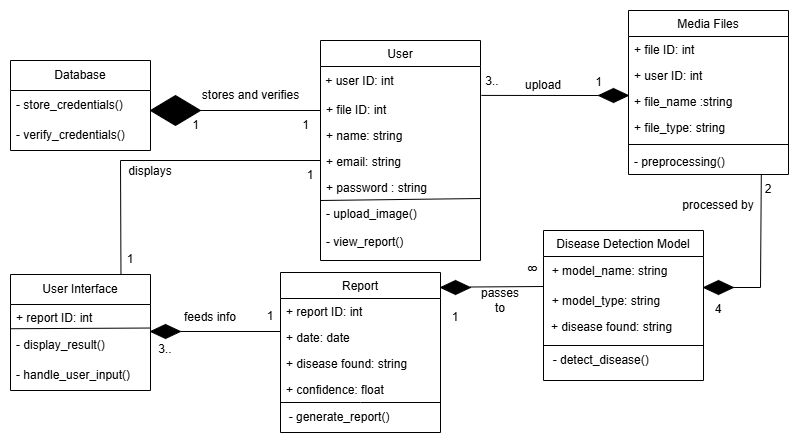
\includegraphics[width=1.0\textwidth]{classdig102.drawio.png}  % Replace with actual image filename
    \caption{Class Diagram}
    \label{fig:class}
\end{figure}

\newpage

% SUBSECTION 5.3: SWIMLANE DIAGRAM
\subsection{Swimlane Diagram}

\vspace{10pt}

An Swimlane Diagram is a structured flow chart that divides a process into multiple lanes, where
each lane is assigned to a specific participant or system component. This structured representation ensures clarity, accountability, and visibility of workflow. In the Ultrasound-Based Clinical
Decision Support System (CDSS), The process begins when the user logs in, triggering ultrasound
image processing. The uploaded image is then analyzed by CNN Model and YOLOv11 Model,
which work together to detect and classify potential diseases. Once the analysis is complete, the
Report System retrieves the processed data, generates a detailed report, and delivers the final diagnostic result to the user. By visualizing these interactions, the Swim Lane Diagram enhances
transparency, making it easier to understand the flow of data between system components while
ensuring efficient processing and accurate diagnosis.

\newpage


\begin{figure}[H] % Changed from [h] to [H] to force placement
    \centering
    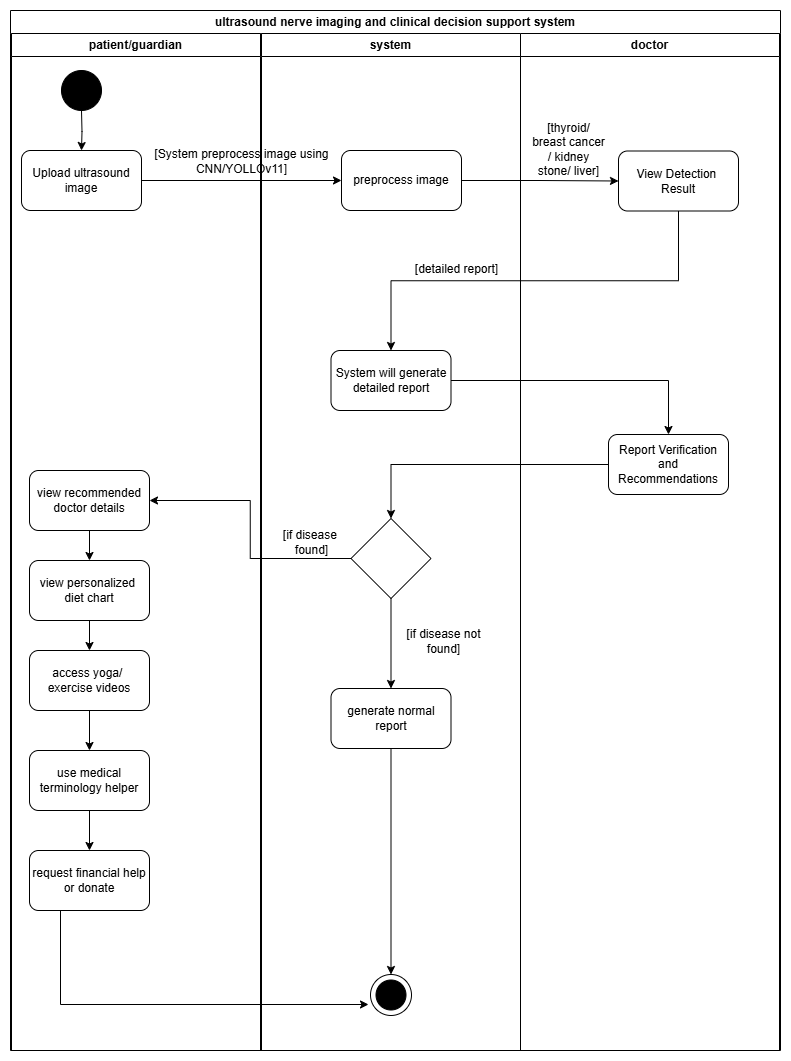
\includegraphics[width=1.0\textwidth, height=0.9\textheight, keepaspectratio]{swimlane101.drawio.png} % Added height and keepaspectratio
    \caption{Swimlane Diagram}
    \label{fig:swimlane}
\end{figure}

\newpage

% SUBSECTION 5.4: SEQUENCE DIAGRAM
\subsection{Sequence Diagram}

\vspace{10pt}

A Sequence Diagram is an interaction diagram that represents the chronological order of messages
exchanged between system components, making it useful for understanding system workflows
and object interactions. In the case of the Ultrasound-Based Clinical Decision Support System
(CDSS), The process begins when the user uploads an ultrasound image. The uploaded image is
then processed by AI models, including CNN and YOLOv11, which analyze the image and classify
any detected diseases. Once the classification is complete, a detailed report is generated containing
the detection results and relevant recommendations. This report is then sent to the user, providing
them with essential diagnostic insights and guidance for further action. This step-by-step message
flow ensures efficient data processing and diagnostic decision-making.

\begin{figure}[h]
    \centering
    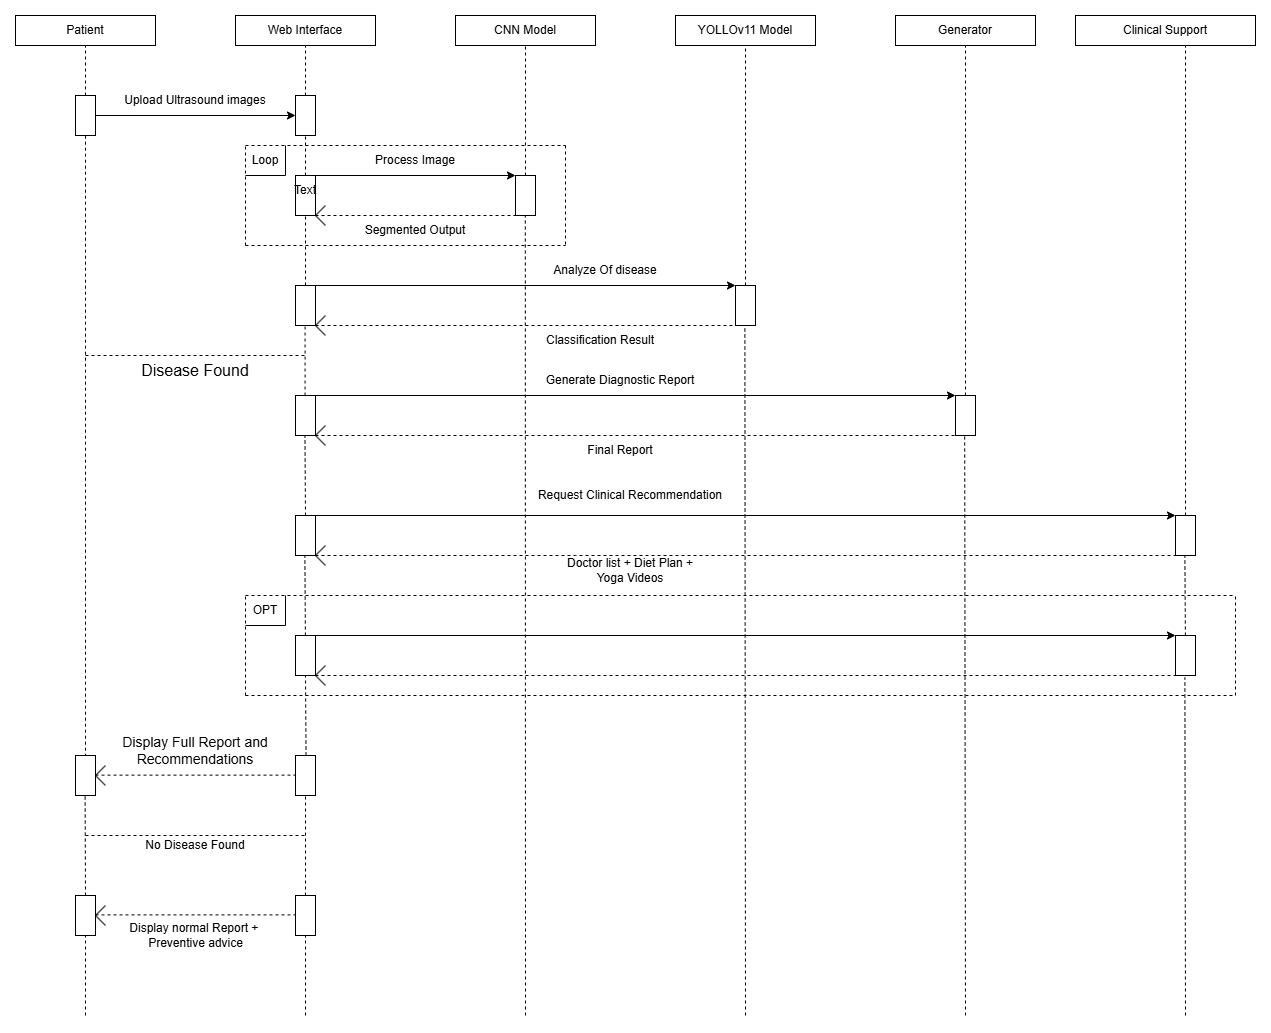
\includegraphics[width=1.02\textwidth]{sequencediagram.drawio (2).png}  % Replace with actual image filename
    \caption{Sequence Diagram}
    \label{fig:sequence}
\end{figure}

\end{document}
